\documentclass[tikz]{standalone}
\usepackage{tikz}

\tikzset{False/.style={circle,draw,fill=gray!10,
                       text badly centered,minimum width=1em}}
\tikzset{True/.style={False,draw,fill=gray!80,}}
                        
%\newcommand{\addsymbol}{\draw[color=magenta] plot[
%            mark=none,
%            samples=100,
%            domain=-3:3,
%        ] ({\x},{1/(1+exp(-\x))});;}
\usepackage{xepersian}
\settextfont[Scale=1]{XB Niloofar}%{B Nazanin}%{Persian Modern}%{XB Nazanin}%
\setlatintextfont[Scale=1]{Times New Roman}
\setdigitfont{Yas}
\defpersianfont\iranic[Scale=.8]{XB Zar Italic}
%\defpersianfont\Keyhan[Scale=1]{XB Kayhan Sayeh}
\defpersianfont\TitleBold[Scale=1.1]{XB Niloofar Bold}
\defpersianfont\AbstractBold[Scale=1]{XB Niloofar Bold}
%\defpersianfont\nastaliq[Contextuals=Swash,Scale=1.2]{IranNastaliq}
\defpersianfont\dimashekasteh[Contextuals=Swash,Scale=1]{Shekasteh_Beta}
\defpersianfont\suls[Contextuals=Swash,Scale=1.2]{A Suls}
%\defpersianfont\dimashekasteh[Contextuals=Swash,Scale=1.2]{Dima Shekasteh Free}
\deflatinfont\mono[Scale=1]{Courier New}

\begin{document}
	    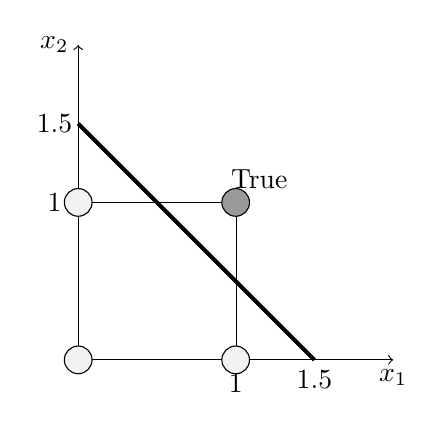
\begin{tikzpicture}[scale=2]
	     \draw[->] (0,0) -- (2,0) coordinate[label = {below:$x_1$}] (x1);
  \draw[->] (0,0) -- (0,2) coordinate[label = {left:$x_2$}] (x2);
  	\node at (1,-0.15) {$1$};
 	\draw [line width=0.5mm] (0,1.5) -- (1.5,0) coordinate[label = {below:$1.5$}];
  	\draw [line width=0.1] (1,0) -- (1,1) -- (0,1);
 	\node at (-0.15,1.5) {$1.5$};
 	\node at (-0.15,1) {$1$};
 	\node[False] at (0,0) {};
 	\node[False] at (0,1) {};
 	\node[False] at (1,0) {};
 	\node[True] at (1,1) {};
 	\node at (1.15,1.15) {\lr{True}};
 	
% 	\draw [line width=0.5mm] (0,1.5) -- (1.5,0) coordinate[label = {below:$1.5$}];
    \end{tikzpicture}
\end{document}